\chapter{State of the art in Distributed Cloud Manufacturing: a Review}
\label{chapter2}
\section{Introduction}
This chapter presents a review of the state-of-the-art in Cloud Manufacturing and its related approaches and enabling key technologies. Techniques used for Cloud Manufacturing design are investigated, followed by a review of Cloud Manufacturing service management aspects. Furthermore, a review of Cloud Manufacturing architectures is provided. The result of this analysis is then used to identify gaps in the research field. This chapter aims to present, in a clear view, a unified picture regarding Cloud Manufacturing, its architectures, and applications. Hence, to provide a holistic view of the phenomena, prior research and frameworks presented in the field relevant to the research question have been analyzed. Therefore, the literature review focuses on two main concepts: cloud manufacturing and cloud manufacturing architectures. The search in academic database engines was limited to keywords related to the research topics.\\
Previous publications, research, and knowledge have been investigated to identify the need for the research and rationalize the research path. An alignment between the research goal and issues that have not been covered satisfyingly has been addressed during the process.\\
The search strings used in the research process are the following:
\begin{enumerate}
    \item TITLE-ABS-KEY("Cloud Manufacturing")
    \item (TITLE-ABS-KEY("Cloud Manufacturing") AND \\ TITLE-ABS-KEY(Architecture) OR TITLE-ABS-KEY(Framework))
\end{enumerate}
To define the inclusion criteria, mentioned search terms were considered, and based on them, a set of search terms were included in the search process. The database search was conducted from 2010 to 2020 since Cloud Manufacturing is an emerging and trending topic. Furthermore, only papers in the English language have been included. Table 1 represents the delimitations, inclusion, and exclusion criteria designed for the first screening stage.\\
\begin{table}
    \centering
    \begin{tabular}{|l|l|}
        \hline
        \textbf{Options} & \textbf{Delimitation}\\
        \hline
        Field & Title, Abstract, Keywords\\
        \hline
        Time & 2010-2020\\
        \hline
        Document Type & Article or Review\\
        \hline
        Language & English\\
        \hline 
    \end{tabular}    

    \caption{Database search delimitations}
    \label{tab:database-search}
\end{table}

The mentioned search terms were used for finding literature based on the inclusion of the search terms in the title, abstract, or keywords section of publications for the first screening stage. For the second screening stage, abstracts of all the selected literature were read to identify publications that might be used in the third stage that included reading through the publications. Table 2 represents the designed guideline for selecting publications after each screening stage in this literature review.
\begin{table}
    \centering
    \begin{tabular}{|c|l|p{4cm}|}
        \hline
        \textbf{Screening Stage} & \textbf{Stage Name} & \textbf{Description}\\
        \hline
        1 & Title Screening & Inclusion of search terms in title, abstract or keywords \\
        \hline
        2 & Abstract Reading & Direct mention of cloud manufacturing context, aspects, implications, concept, algorithms, paradigms methods and/or models in the abstract \\
        \hline
        3 & Full Text Screening & Relevance and contribution to the aim of the research and the research questions \\
        \hline
    
\end{tabular}

    \caption{Publications selection process after each screening stage}
    \label{tab:pub-sel-process}
\end{table}

In the first part of the literature review, the focus was on Cloud Manufacturing and its types, characteristics, and attributes. The results from this phase are the following:
\begin{itemize}
    \item Understand the cloud manufacturing concept by exploring various definitions of Cloud Manufacturing.
    \item Show latest Cloud Manufacturing frameworks.
    \item Identify Cloud Manufacturing key architectural factors.
    \item Detect Cloud Manufacturing research challenges and gaps.
\end{itemize}

\section{Cloud Manufacturing}
The development of new advanced manufacturing modes with the flexibility to suit the market is becoming one of the main trends of the manufacturing industry nowadays. A number of advanced manufacturing models, such as Agile Manufacturing \parencite{yy_yusuf_agile_1999}, Virtual Manufacturing \parencite{souza_virtual_2006}, and Networked Manufacturing, are flourishing in this context. Cloud Manufacturing was introduced in 2010 to overcome the impediments to applying Networked Manufacturing and solve more complex manufacturing problems and perform larger-scale collaborative manufacturing \parencite{bo-hu_cloud_2010}.\\
The evolution of key enabling technologies brought a growing unpredictability of the markets, and with increased competition, manufacturing systems boundaries are extended from a factory towards new kinds of network relationships. As a result, enterprises’ mission and business strategy have also changed, e.g., from product competitive advantage towards collaborative added value, and the way enterprises perform business have been transformed \parencite{chituc2009challenges}. Consequently, a wide range of different paradigms emerged, such as Lean Manufacturing, Agile Manufacturing, Flexible Manufacturing, reconfigurable manufacturing systems, distributed virtual manufacturing systems.\\
Agile Manufacturing systems are designed to respond to customer and market changes quickly. Although lean and agile manufacturing concepts sound similar, they have different approaches to manufacturing engineering systems. While Lean Manufacturing responds to competitive pressure with limited resources, agile Manufacturing represents the response to complexity brought about by constant change. Flexible manufacturing systems are manufacturing systems designed to rapidly adjust their production capacity and functionality in response to new circumstances by rearranging or changing their components. Networked Manufacturing systems combine advanced manufacturing technologies with network technology to introduce Distributed Manufacturing systems through the Internet. Networked Manufacturing models provide information and resource sharing among enterprises but lack direct access to physical resources, nor does it achieve the dynamic intelligent sharing and distribution of manufacturing resources. Intelligent manufacturing systems bring those features. These are manufacturing systems enhanced with human-like capabilities \parencite{chituc2009challenges}. Cloud manufacturing is emerging as a manufacturing paradigm that combines most of the development from previous models and attempts to solve most of their drawbacks, attracting experts, scholars, and enterprises. Cloud Manufacturing is promising in transforming today’s manufacturing industry towards service-oriented, highly collaborative, and innovative Manufacturing in the future \parencite{ren_cloud_2017}. Cloud Manufacturing is the result of adopting key enabling technologies (such as Industrial Internet of Things, Cloud Computing, Digital Twins, Big Data) by manufacturing enterprises to share resources and capabilities to enhance their response to market requirements and increase cost effectiveness \parencite{ren_cloud_2015}. The advantages of Cloud Manufacturing make it a new field of research.

\begin{table}
    \centering
    \begin{tabular}{|p{2cm}|p{2cm}|p{3cm}|p{3cm}|}
        \hline
         & \textbf{Flexible manufacturing} & \textbf{Distributed (Network) manufacturing} & \textbf{Cloud manufacturing}\\
         \hline
         \textbf{System functions} & Cooperation & Resource sharing/cooperation  & Resource sharing/resource efficiency/cooperation \\
         \hline
         \textbf{System openness} & Many constraints, poor openness & Better openness & Highly open \\
         \hline
         \textbf{Resource type} & Organization, human, technology & Equipment, people, materials, network, information & Materials, equipment, software, hardware, logistics, human, knowledge \\
         \hline
         \textbf{Resource usage} & Customization & Dynamic configuration & On-demand dynamic configuration \\
         \hline
         \textbf{Collaboration scope} & Several companies & Companies in several industries & Companies in almost every industry \\
        \hline
    \end{tabular}
    \caption{Comparison of characteristics of three advanced manufacturing models, author’s elaboration from \textcite{wei_product_2020}}
    \label{tab:comp-adv-mfg-models}
\end{table}

In conclusion, the analysis of the state-of-the-art has highlighted three key trends in the evolution of manufacturing systems: (i) reconfigurability; (ii) lowering complexity; (iii) increase the need for autonomy. In addition, from the latest Smart Manufacturing techniques that mimic human-like capabilities, four interesting key factors are commonly presented in manufacturing systems:
\begin{itemize}
    \item self-configuration: from low level (machine) to high level (plant), the system needs to be able to drastically adapt and change
    \item self-optimization: automated optimization methods to increase overall utilization
    \item self-protection: being able to anticipate possible threats and provide counteractions for the short and long term
\end{itemize}

\section{Towards a common definition}
The concept of Cloud Manufacturing was first proposed by Li Bo-Hu in China \parencite{bo-hu_cloud_2010} and it is defined as a new networked manufacturing model that is able to solve more complex manufacturing problems and perform larger- scale collaborative manufacturing through the introduction of key enabling technologies (such as cloud computing, cloud security, high-performance computing, Internet of things) in a new service-oriented model. In this model, scattered online manufacturing resources are structured in a platform where users can access eligible manufacturing services. While Cloud Manufacturing is a relatively new concept, a variety of definitions are present in the literature from scholars that have modified and enhanced it; a selection is listed below:
\begin{itemize}
    \item “A customer-centric manufacturing model that exploits on-demand access to a shared collection of diversified and distributed manufacturing resources to form temporary, reconfigurable production lines which enhance efficiency, reduce product lifecycle costs and allow for optimal resource loading in response to variable- demand customer-generated tasking” \parencite{wu_cloud_2013}.
    \item “A model for enabling ubiquitous, convenient, and on-demand network access to a shared pool of configurable manufacturing resources (e.g., manufacturing software tools, manufacturing equipment, and manufacturing capabilities) that can be rapidly provisioned and released with minimal management effort or service provider interactions” \parencite{xu_cloud_2012}.
    \item “A new-generation service-oriented approach to supporting multiple companies to deploy and manage services for manufacturing operations over the Internet” \parencite{vincent_wang_interoperable_2013}.
    \item “A new networked manufacturing model which aims at achieving low- cost resource sharing and efficient coordination. It transforms all kinds of manufacturing, simulation, and computing resources and abilities into manufacturing services to form a huge manufacturing cloud and distributes them to users on-demand” \parencite{laili_study_2012}.
\end{itemize}

\textcite{xu_cloud_2012} expanded the original scope of “online manufacturing resources” from \textcite{bo-hu_cloud_2010} including manufacturing capabilities along with manufacturing resources. In order to access such manufacturing resources, \textcite{tao_cloud_2011} and \textcite{ren_cloud_2017} emphasized the importance of key enabling technologies in the definition of Cloud Manufacturing from ICT (such as Machine Learning, Big Data, 5G) and manufacturing technologies (such as Additive Manufacturing, Intelligent Robots, and Intelligent Manufacturing techniques). From an organizational point of view, an interesting addition to the Cloud Manufacturing definition is brought by \textcite{wu_cloud_2013} where on-demand services are seen as a trigger to create instant, reconfigurable networks to respond to complex and variable task requirements from the market. Another important addition that widens the definition of Cloud Manufacturing comes from the work of \textcite{fisher_cloud_2018} where the authors, after a detailed comparison of Cloud Manufacturing key characteristics and a deep analysis of the future of manufacturing systems, identify Cloud Manufacturing as a route to Sustainable Manufacturing. Finally, \textcite{tao_cloud_2011} clarified the origin of Cloud Manufacturing. While this is a new service-oriented model, Cloud Manufacturing is an evolution from existing advanced manufacturing models presented in the previous paragraphs (such as agile manufacturing, networked manufacturing, manufacturing grid). In other words, other research on this topic exists but presents slightly different viewpoints. Cloud Manufacturing can promote collaborative design techniques by sharing design information. Cloud Manufacturing, if correctly implemented,can also enhance resource sharing, rapid production of prototypes, and reduce costs. Distributed manufacturing can be developed as a result, although resource autonomy and system governance have not been addressed. Cloud Manufacturing can potentially reduce time-to-market, improve service, and enhance user experience, which advantageously impacts customer co-creation area \parencite{wu_cloud_2013-1}. While \textcite{adamson_state_2013} outlined that Cloud Manufacturing is not always a feasible solution for enterprises, mainly due to lack of competencies for its implementation, \parencite{wu_economic_2015} identified the key economic benefits required for a comparative study that supports organizations in determining when traditional in-house design and manufacturing versus CBDM is most appropriate. The study explored key factors of a cost-benefit analysis through a cost breakdown and a price comparison with cloud computing pricing plans on different levels (e.g., IaaS, Paas, SaaS). \parencite{wu_cloud_2013-1}, in another study, showed three sectors that could be affected by cloud manufacturing on long and short terms: (i) the engineering and design sector; (ii) the manufacturing sector; and (iii) the marketing and service sector. Explicitly, In the short term, Cloud Manufacturing can offer ubiquitous access to design information, improve efficiency, adequate computing resources for the engineering and design sector, thus producing a collaborative design approach in the long term.\\
In the manufacturing sector, the Cloud Manufacturing environment can potentially improve resource sharing, rapid prototyping, and reduction in costs, hence improving distributed manufacturing in the long term. As for the marketing and service sector, time to market can be reduced, service quality can be improved, and customer needs elicitation can potentially be enhanced. Consequently, cloud manufacturing can possibly provide a customer co-creation environment \parencite{mourad_assessment_2020}.\\
Throughout these insights, cloud manufacturing would thus play a significant role in the development and execution of product lifecycle processes, as in cloud manufacturing; product life cycle activities and functions can be supported by virtualized manufacturing resources and the manufacturing capabilities layer allocated within the cloud manufacturing system. Thus, this can allow more users to access these services, delegating the manufacturing enterprises (service provider) to carry out all activities (processes) involved in the entire life cycle of the product and to focus only on their core business and services \parencite{tao_cloud_2011}.

\section{Cloud Manufacturing Architectures}
The architecture of Cloud Manufacturing is the system design planning for Cloud Manufacturing implementation and the basis for the development and application of a Cloud Manufacturing actual system; the supporting technologies of Cloud Manufacturing are the foundation for realizing the Cloud Manufacturing architectures and supporting the completion of Cloud Manufacturing business; the phased application status analysis of the Cloud Manufacturing is the reference for finding the problems and deficiencies in the development of Cloud Manufacturing. Therefore, an effective exploration of the current research status in terms of architecture, supporting technologies, application status of Cloud Manufacturing plays a vital role in the innovation of its theory, technology, and application development \parencite{lim_theory_2020}. Various models are used to describe the architecture of a Cloud Manufacturing platform. The most commonly used is based on a multi- layered architecture with a modular approach from \parencite{he_state---art_2015}, where each layer presents a specific role that accomplishes the required functions. In this paragraph, a variety of Cloud Manufacturing architectures are depicted to embrace the similarities and contrast between them and further to be a baseline for the development of this research.\\
\textcite{ding_cloud-based_2012} proposed a layered framework of collaborative manufacturing resources shared based on cloud services. The study designs an architecture with three main layers: (i) Cloud service demand layer; (ii) Cloud service center; (iii) Cloud service provider layer. Each layer is composed of more specific sub-layers. The cloud service demand layer is based on the Cloud user interface. Layer (i) is connected to layer (ii) through an application interface. Layer (ii) provides a variety of core services and function and is divided into two sub-layers: (a) Cloud service management, responsible for user management, task management (publication, aggregation, scheduling), service search; (b) Cloud service integration, provides integration and semantic interoperability of a wide range of manufacturing resources through a global and a local service integration model. A Cloud access interface is a gateway that allows multiple manufacturing resources from the Cloud service provider layer (iii) to work with the layer (ii).

\begin{figure}[h]
    \centering
    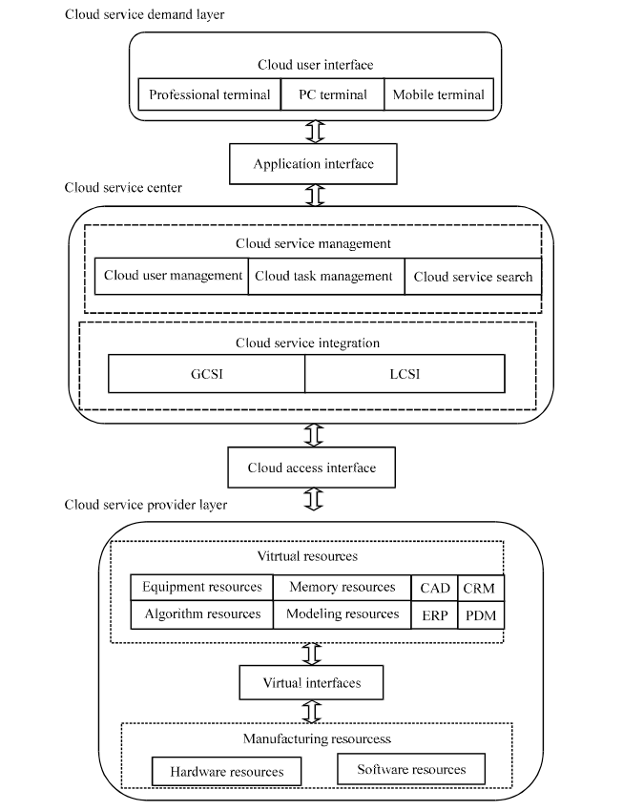
\includegraphics[height=4cm, keepaspectratio]{images/ding-three-layer-architecture}
    \caption{\textcite{xu_cloud_2012} three-layer architecture for CMfg}
    \label{fig:ding-3-layer-architecture}
\end{figure}

Moreover, \textcite{wei_jiang_research_2012} introduced a five-layered structure based on collaborative agents (CAgents) with the following layers: (a) basement layer (b)access layer (c)functional layer (d)portal layer (e) application layer. The functional layer is responsible for controlling and coordinating the various service transactions within the cloud manufacturing system.

\begin{figure}[h]
    \centering
    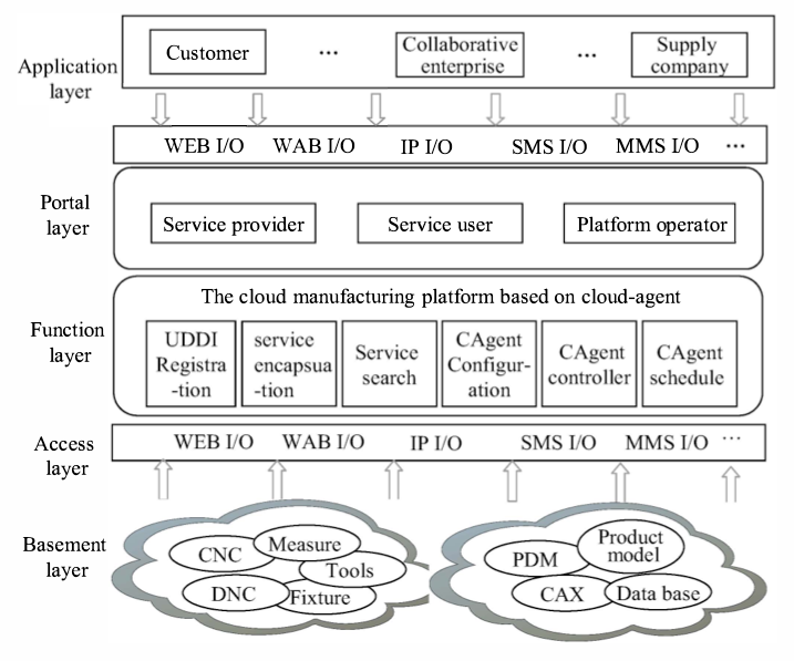
\includegraphics[height=4cm, keepaspectratio]{images/jiang-cloud-mfg}
    \caption{\textcite{wei_jiang_research_2012} cloud manufacturing integrated service platform based on CAgent}
    \label{fig:jiang-architecture}
\end{figure}

\textcite{li_icms_2013} expands the role of the Master Cloud Agent within the smart cloud manager layer to analyze, optimize and control the Cloud Manufacturing service interactions between the user layer and the manufacturing capability.

\begin{figure}[h]
    \centering
    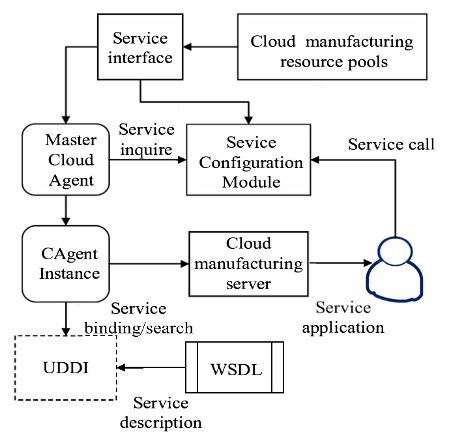
\includegraphics[height=4cm, keepaspectratio]{images/wang-integrated-mfg-services}
    \caption{\textcite{li_icms_2013} - The integrated manufacturing service mode based on cloud agents}
    \label{fig:ding-3-layer-architecture}
\end{figure}

\textcite{lv_multi-view_2012} proposed another typical four-layered hierarchy architecture. This architecture offers a more detailed mapping of resource entities into cloud services from physical resource layer to virtual resource layer, which highlights the core idea of an open cloud service architecture. The architecture is based on a multi-view model that integrates different views (function view, resource view, information view, and process view), with each view depicting a different aspect of the platform.


\begin{figure}[h]
    \centering
    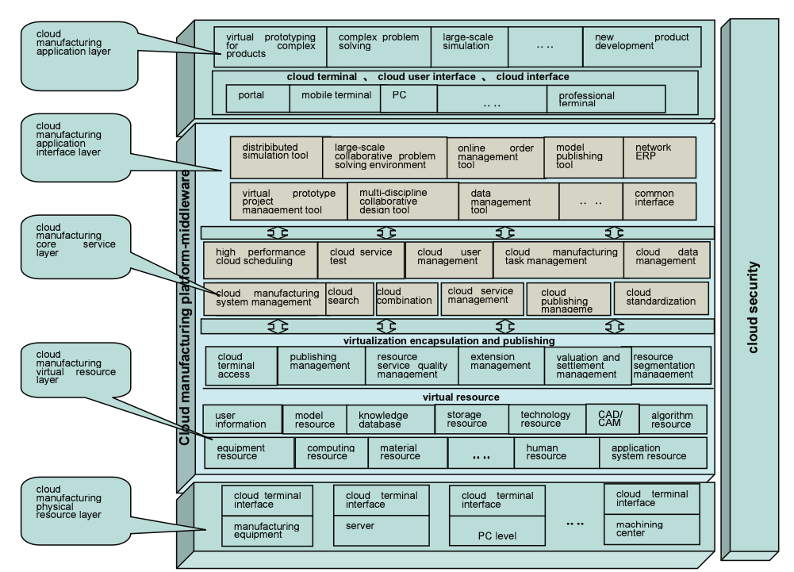
\includegraphics[height=4cm, keepaspectratio]{images/lv-cmfg-architecture}
    \caption{\textcite{lv_multi-view_2012} Cloud Manufacturing Architecture}
    \label{fig:lv-cmfg-architecture}
\end{figure}

The function view lists the various tasks that a system can perform and comprises interlinked activities. The resource view enumerates the resources required to perform activities. The information view focuses on the required data for the activities, and the process view captures the sequence of the activities.

\begin{figure}[h]
    \centering
    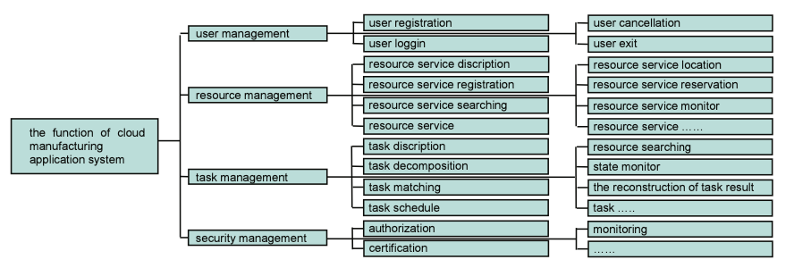
\includegraphics[height=4cm, keepaspectratio]{images/lv-cmfg-function-tree}
    \caption{\textcite{lv_multi-view_2012} Cloud Manufacturing System function tree}
    \label{fig:lv-cmfg-function-tree}
\end{figure}


Moreover, a novel approach that is not mainly focused on technical aspects of the Cloud Manufacturing system comes from \textcite{skulj_decentralised_2015} that proposed a decentralized perspective for a cloud manufacturing architecture (CMdna) shown in Figure 8. One of the main contributions of this work derives from the introduction of the concept of a cloud manager component (layer) with the aim of creating a flexible connection between cloud service providers and service users through the utilization of autonomous work systems (AWS) that acts as numerous manufacturing clouds which vary depending on the requirements of both service users and service providers. Such an architecture would allow several clouds to bid for each stage of the required work to make the process as cheap as possible for the end-user.

\begin{figure}[h]
    \centering
    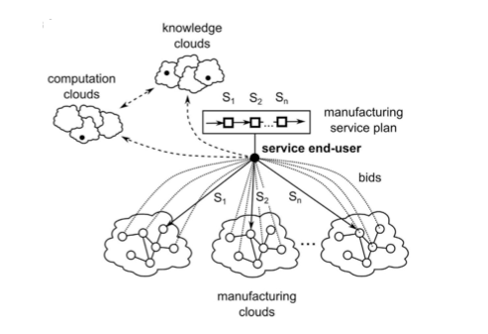
\includegraphics[height=4cm, keepaspectratio]{images/skulj-cmdna}
    \caption{\textcite{skulj_decentralised_2015} - Decentralized Cloud Manufacturing Network}
    \label{fig:skulj-cmdna}
\end{figure}

Based on the proposed architectures and considering the similarities of the models presented in the literature, a novel architecture is proposed on Chapter III to overcome issues not tackled by the typical configuration of the cloud manufacturing systems as depicted on Chapter II Section 5.

/section{Cloud Manufacturing Service Managemen}
Services Management within Cloud Manufacturing is considered a critical issue. Indeed, an important goal of Cloud Manufacturing is to provide users with on-demand services for the manufacturing resources and capabilities they need. After these distributed and heterogeneous resources are virtualized, modelled, and transformed into services on the cloud, there is a solid need to effectively manage and coordinate these services in a centralized way to ensure the service performance, quality, security, and successful operation of manufacturing clouds \parencite{he_state---art_2015}. Resources can interact into a public cloud or a private cloud based on the difference in service object \parencite{zhang_cloud_2014}. In order to ensure service performance of Cloud Manufacturing, various methods have been proposed. \textcite{model_information_2012} developed a system based on an ontology of virtualized manufacturing resources. \textcite{liu_resource_2011} proposed three multi-agent systems architectures for different enterprise sizes. The three architecture are the following and mainly diversified by the role of the Master Agent:
\begin{itemize}
    \item (a) the Facilitator Architecture: The facilitator is a special agent responsible for coordinating the communication among the agents. The facilitator provides a reliable communication layer, routes messages among agents based on the contents of the messages, and coordinates the control of the multi-agent activities. All the agents in a facilitator-centric architecture communicate with each other via the facilitator. As a result, the robustness of this architecture can be poor, and the overhead is relatively high.
    \item (b) The Mediator Architecture: As the facilitator, the mediator is a special agent with more functions than the facilitator. Besides coordinating the communication among the agents and the control of the multi-agent activities, the mediator is able to search for relevant agents according to the agents’ requirements and assist in setting up communication among them. All the agents in a mediator-centric architecture communicate with each other through the mediator. However, the agents can also communicate with each other after the communication has been set up (indicated as dotted lines). In contrast to the facilitator-centric architecture, the overhead of the mediator-centric Multi-Agent System is reduced.
    \item (c) The Autonomous Agent Architecture: As the facilitator, the mediator is a special agent with more functions than the facilitator. Besides coordinating the communication among the agents and the control of the multi-agent activities, the mediator is able to search for relevant agents according to the agents’ requirements and assist in setting up communication among them. All the agents in a mediator-centric architecture communicate with each other through the mediator. However, these agents can also communicate with each other after the communication has been set up (indicated as dotted lines). In contrast to the facilitator-centric architecture, the overhead of the mediator- centric MAS is reduced.
\end{itemize}


\begin{figure}[h]
    \centering
    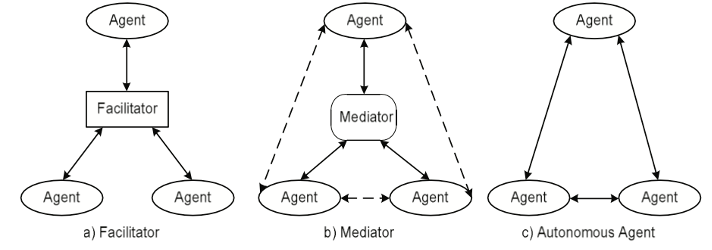
\includegraphics[height=4cm, keepaspectratio]{images/liu-mas-architecture}
    \caption{MAS Architecture proposed by \textcite{liu_resource_2011}}
    \label{fig:liu-mas-architecture}
\end{figure}

Several studies have examined service quality and composition in a Cloud Manufacturing platform. \textcite{lin_oics_2015} introduced an Ontology inference cloud service (OICS). An OICS is a knowledge-based cloud manufacturing system and is used to recommend machine tools and cutting tools based on the Ontology inference techniques for cloud services. The OICS comprises three core functional modules: The Ontology inference module, the VMT (Virtual Machine Tool) module, and the request filtering module. Modules are developed to allow multiple users to perform inference service and verify the recommended machine tools or cutting tools via VMT simulations. The proposed system provides the optimal number of machine tools for the acquired system based on the designed ontology data of the system and thus aims to improve the quality of the cloud manufacturing services.\\
Finally, Lu proposed a knowledge-based service composition and adaptive resource planning model in a cloud manufacturing environment in order to develop an integrated networked environment enabling the optimal allocation of resources based on given criteria. The model is deployed as a web service and is based on three critical stages: (a) collaborative business process modelling and verification of cloud workflow; (b) model instantiation with modelling and clustering of manufacturing services; (c) model execution, with the optimal matching of manufacturing service supplies and requirements.

\section{Research Gap Analysis}
Cloud Manufacturing can potentially present a strong impact on manufacturing systems. However, further investigation is still required to identify the communication and interaction protocols of the cooperative systems that enable the integration of service providers and service users. The most important gap identified by the author, however, is not in the constituent parts of the cloud (as many cyber physically enabled smart manufacturing components already exist), the protocols (as plenty of excellent work has been done in this area already), or the integration (as the researchers have proposed several approaches likely to succeed). Architecture designs that are presented in literature reflect the cognition and expectation of different researchers. While most architectures found in the literature are characterized by functional views and resource-based views, articulated in a multi-layer structure, almost none presents a process and organizational view. While most architectures assume direct access and control of the scattered physical resources, only \textcite{skulj_decentralised_2015} proposes an architecture based on Autonomous Work Systems. Finally, while Cloud Manufacturing works presents multiple efforts on service optimization, almost none deals with the negotiation of service allocation with service providers. Services created by aggregating autonomous service providers represent a step forward in an architecture that fits actual enterprise characteristics (especially Small and Medium Enterprises) and better applicability in real-world cases.\\
The author believes that the main research gap in Cloud Manufacturing architectures is in the characteristics of Service Providers. The presence of autonomous and platform-independent manufacturing resources brings numerous issues derived from a distributed governance. Additionally, the literature shows that other gaps in Cloud Manufacturing research are present. Other research gaps identified include:
\begin{enumerate}
    \item A lack of research directed towards the platform implementation: most scholars have concentrated only on Cloud Manufacturing architecture and its enabling technologies: there is a need to examine Cloud Manufacturing with real case studies to demonstrate the usability and successful implementation in a real-life context.
    \item A lack of research work from the managerial point of view in cloud manufacturing: there are many studies regarding the technical issues around Cloud Manufacturing in the literature. These studies have typically overlooked how to manage cloud manufacturing from a management point of view. Issues that need to be addressed include stakeholders’ interactions and their activities, the cloud’s standards, services management, utility models, servitization technologies, and the role of clear and shared founding principles in a Cloud Manufacturing platform.
    \item A lack of research regarding how to manage negotiation in cloud manufacturing: the literature reveals that there is not yet an understanding of negotiation mechanisms for cloud manufacturing. There is a need to identify, assess, and control interactions among service demanders and service providers inside the network.
\end{enumerate}

Therefore, this research proposes an architecture of a distributed Cloud Manufacturing network comprised of autonomous service providers to manage operations and coordinate communications among manufacturing nodes and service providers. The aim is to offer new insights for industry and academia on how to deal with autonomous service providers at the adoption and implementation stages of the platform.
